\chapter{Malware e file Windows PE}

\section{Il formato Windows PE}

Il Portable Executable (PE) è il formato utilizzato nei sistemi Windows
per i file \texttt{.exe}, \texttt{.dll} e altre tipologie di file
eseguibili. Inizialmente progettato come formato eseguibile standard
per i sistemi Windows, il formato PE, fin dalla sua introduzione, ha
subito diverse modifiche, anche in seguito al passaggio ai sistemi
Windows a 64 bit.

La struttura di un file PE contiene le informazioni necessarie al
sistema operativo Windows per caricare e gestire il codice eseguibile.
Oltre al codice da eseguire, un file PE contiene infatti metadati e
altre informazioni organizzate secondo una struttura ben definita,
la cui conoscenza riveste un ruolo importante nell'ambito dell'analisi
dei malware.

In particolare, la struttura di un file PE è organizzata in tre parti
principali \cite{microsoftPE}, come mostrato nella
Figura~\ref{fig:pe_structure}:

\begin{itemize}
    \item \textbf{Header}: contiene le informazioni principali relative
    al file PE e al suo caricamento in memoria. L'header è a sua volta
    suddiviso nelle seguenti parti:

    \vspace{-0.5em}
    \begin{itemize}
        \item \textbf{DOS Header}: rappresenta la parte iniziale del file PE
        e contiene informazioni relative al formato DOS. Contiene inoltre un
        riferimento che indica la posizione iniziale del PE Header;

        \item \textbf{DOS Stub}: viene utilizzato per visualizzare un messaggio
        che indica se il programma può essere eseguito o meno in modalità DOS;

        \item \textbf{NT Header}: contiene le principali informazioni
        relative al file PE ed è a sua volta suddiviso in:

        \begin{itemize}
            \item \textbf{PE Signature}: identifica il file come Portable
            Executable;

            \item \textbf{COFF File Header}: contiene informazioni sulle
            caratteristiche del file e sulle sezioni presenti;

            \item \textbf{Optional Header}: contiene informazioni utilizzate
            durante il caricamento del file in memoria, tra cui il punto di
            ingresso del programma.
        \end{itemize}
    \end{itemize}

    \item \textbf{Tabella delle sezioni}: descrive le caratteristiche delle
    diverse sezioni presenti nel file e contiene le informazioni necessarie
    per mapparle in memoria e indicare se ciascuna sezione è di sola lettura
    oppure scrivibile;

    \item \textbf{Sezioni}: contengono il codice e i dati del file PE.
    Tra le sezioni comunemente presenti si trovano:

    \begin{itemize}
        \item \texttt{.text}: contiene il codice eseguibile;

        \item \texttt{.data}: contiene le variabili globali e statiche
        inizializzate;

        \item \texttt{.bss}: contiene le variabili globali e statiche
        non inizializzate;

        \item \texttt{.rsrc}: contiene le risorse utilizzate dal programma,
        come icone, immagini, stringhe e finestre di dialogo;

        \item \texttt{.reloc}: contiene i dati necessari alla rilocazione
        del programma;
    \end{itemize}
\end{itemize}

\begin{figure}[!ht]
    \centering
    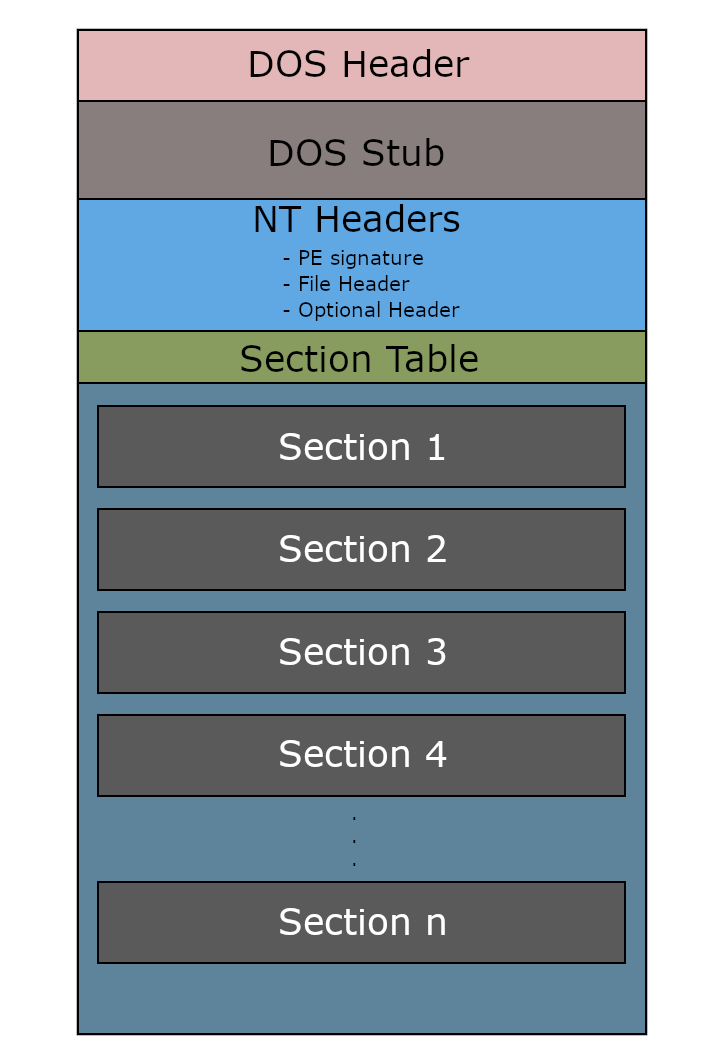
\includegraphics[width=0.6\textwidth]{images/pe_structure.png}
    \caption{Struttura generale di un file PE, tratta da \cite{khan2023}}
    \label{fig:pe_structure}
\end{figure}

\FloatBarrier

L'header riveste un ruolo importante nella classificazione dei malware,
dato che le informazioni in esso contenute sono risultate tra quelle
che contribuiscono maggiormente al processo di classificazione
\cite{zhang2024}.

L'analisi della struttura delle sezioni può essere utile anche
nell'ambito del rilevamento dei malware, dato che il codice malevolo
può essere nascosto all'interno di sezioni insolite oppure possono
essere aggiunte ulteriori sezioni con l'obiettivo di rendere più
complessa l'analisi del file. Inoltre, i file malware possono presentare
anomalie nella struttura e nelle caratteristiche del formato PE rispetto
ai file benigni, rendendo queste informazioni rilevanti per il loro
rilevamento \cite{bai2014}.

\vspace{0.5cm}

\section{Malware e tecniche di rilevamento}

Il termine malware deriva da \textit{malicious software} e indica
un software progettato con lo scopo di compromettere la riservatezza,
l'integrità o la disponibilità dei dati, delle applicazioni o del
sistema operativo \cite{souppaya2013}.

I malware possono essere suddivisi in diverse tipologie in base alle
loro caratteristiche e al loro comportamento. Inoltre, queste categorie
non sono esclusive, poiché uno stesso malware può presentare
contemporaneamente caratteristiche appartenenti a più tipologie
\cite{egele2012}.

Tra le principali tipologie di malware abbiamo i \textit{worm}, che
sono programmi in grado di essere eseguiti in modo indipendente e con
la capacità di propagarsi verso altri sistemi. I worm possono inoltre
essere utilizzati per creare \textit{botnet}, impiegate per l'invio
di messaggi di spam o per effettuare attacchi di tipo Distributed
Denial of Service (DDoS), nei quali più computer infettati da worm
agiscono in modo coordinato per esaurire le risorse di un sistema o
la sua banda di rete.

I \textit{virus}, a differenza dei worm, non possono essere eseguiti
in modo indipendente, ma inseriscono il proprio codice malevolo
all'interno di altri programmi e si attivano quando viene eseguito
il programma infettato. Possono inoltre propagarsi infettando altri
file presenti nel sistema e, attraverso file presenti su server
condivisi, diffondersi anche verso altri computer.

I \textit{Trojan horse} sono programmi che si presentano come software
legittimi, ma che eseguono operazioni malevole in background. Una volta
installati, possono ad esempio scaricare altri malware, modificare le
impostazioni del sistema o infettare altri file.

Gli \textit{spyware} sono malware utilizzati per raccogliere informazioni
sensibili dal sistema infetto e trasmetterle all'attaccante. Le
informazioni raccolte possono comprendere credenziali di accesso,
dati bancari, pagine web visitate oppure il contenuto di documenti
ed e-mail.

I \textit{bot} permettono a un attaccante, chiamato \textit{bot master},
di controllare da remoto il sistema infetto. Un insieme di bot
controllati dallo stesso \textit{bot master} costituisce una
\textit{botnet}, che può essere utilizzata, ad esempio, per l'invio
di messaggi di spam o per attività di spyware.

Infine, i \textit{rootkit}, la cui principale caratteristica è quella
di nascondere determinate informazioni all'utente del sistema, come
processi, file o connessioni di rete. Per questo motivo, molti malware
utilizzano tecniche proprie dei rootkit per nascondere la propria
presenza all'interno del sistema.

Il rilevamento dei malware può essere effettuato attraverso diverse
tecniche. Uno degli approcci tradizionalmente utilizzati, anche dagli
antivirus, è quello basato sulle firme, in cui i file vengono confrontati
con un insieme di firme associate a malware già conosciuti.

Questo approccio presenta tuttavia alcuni limiti, in particolare le firme
vengono generalmente create da analisti, richiedendo tempo e potendo
essere soggette a errori. Inoltre, i metodi basati sulle firme non sono
in grado di rilevare minacce sconosciute per le quali non è ancora
disponibile una firma, dato che solo quando viene individuata una nuova
minaccia questa può essere analizzata e può essere creata una nuova
firma, che viene successivamente aggiunta al database utilizzato per
il rilevamento \cite{egele2012}.

Per affrontare alcuni dei limiti dei metodi basati sulle firme, sono
state sviluppate altre tecniche per il rilevamento dei malware. In
particolare, è possibile distinguere due principali approcci:
l'analisi dinamica e l'analisi statica, in base all'esecuzione o meno
del programma durante la raccolta delle feature, ovvero delle
caratteristiche utilizzate per effettuare l'analisi
\cite{zhang2024}.

\begin{figure}[!ht]
    \centering

    \begin{tikzpicture}[
        node distance=0.7cm and 1.2cm,
        main/.style={
            draw,
            rounded corners=2pt,
            align=center,
            minimum height=0.9cm,
            text width=4.2cm
        },
        title/.style={
            draw,
            rounded corners=2pt,
            align=center,
            minimum height=0.9cm,
            text width=4.2cm,
            font=\bfseries
        },
        arrow/.style={
            -{Latex[length=2mm]},
            thick
        }
    ]

        % Titolo
        \node[title] (analysis)
        {Analisi dei malware};

        % Due approcci
        \node[title, below left=0.8cm and 0.7cm of analysis]
        (dynamic)
        {Analisi dinamica};

        \node[title, below right=0.8cm and 0.7cm of analysis]
        (static)
        {Analisi statica};

        % Esecuzione
        \node[main, below=of dynamic]
        (dynamicExecution)
        {Programma in esecuzione};

        \node[main, below=of static]
        (staticExecution)
        {Programma non eseguito};

        % Informazioni analizzate
        \node[main, below=of dynamicExecution]
        (dynamicInformation)
        {Comportamento del programma};

        \node[main, below=of staticExecution]
        (staticInformation)
        {Contenuto del file};

        % Feature
        \node[main, below=of dynamicInformation]
        (dynamicFeatures)
        {Chiamate API\\
        Comunicazioni di rete\\
        Memoria e CPU};

        \node[main, below=of staticInformation]
        (staticFeatures)
        {Rappresentazione binaria};

        % Frecce
        \draw[arrow] (analysis) -- (dynamic);
        \draw[arrow] (analysis) -- (static);

        \draw[arrow] (dynamic) -- (dynamicExecution);
        \draw[arrow] (static) -- (staticExecution);

        \draw[arrow] (dynamicExecution) -- (dynamicInformation);
        \draw[arrow] (staticExecution) -- (staticInformation);

        \draw[arrow] (dynamicInformation) -- (dynamicFeatures);
        \draw[arrow] (staticInformation) -- (staticFeatures);

    \end{tikzpicture}

    \caption{Confronto tra analisi dinamica e analisi statica dei malware,
    basato su \cite{zhang2024}}
    \label{fig:static_dynamic_analysis}
\end{figure}

L'analisi dinamica prevede l'esecuzione del programma e l'osservazione
del suo comportamento durante l'esecuzione. In questo modo possono
essere raccolte diverse informazioni, tra cui le sequenze delle
chiamate API, le comunicazioni di rete, lo stato della memoria e
della CPU. Questo tipo di analisi può inoltre contribuire al
rilevamento di malware precedentemente sconosciuti e risulta meno
vulnerabile alle tecniche di offuscamento del codice. 

Tuttavia, presenta alcuni limiti, dato che ogni campione deve essere
eseguito per un determinato periodo di tempo e può essere analizzato
un singolo percorso di esecuzione del programma \cite{bai2014}.

A differenza dell'analisi dinamica, l'analisi statica permette di
analizzare un programma senza eseguirlo e, per questo motivo, richiede
tempi inferiori per l'analisi. Dato che generalmente il codice sorgente
dei malware non è disponibile, le tecniche di analisi statica
applicabili devono ricavare le informazioni direttamente dalla
rappresentazione binaria del programma.

Anche l'analisi statica presenta alcuni limiti, dato che lavorare
direttamente sulla rappresentazione binaria di un programma può
risultare complesso. Inoltre, i malware possono utilizzare tecniche
in grado di modificare il programma e ostacolare questo tipo di
analisi \cite{egele2012}.

I limiti degli approcci descritti in precedenza, insieme alla crescente
complessità e quantità dei malware, hanno favorito l'utilizzo di
tecniche basate sul Machine Learning. In particolare, queste tecniche
permettono di apprendere modelli e pattern a partire dalle feature
estratte dai malware, con l'obiettivo di supportarne il rilevamento
e l'analisi \cite{ucci2019}.